%Author: Michael Bucher
\section{Host Client}

The Host Client is a web-based application for event hosts to edit, track and create events. The application contains one component that is displayed and runs all the time. This component contains a navigation that routes between the five views of the application. To do so, it contains a navigation component on top with a sidebar that can be opened and closed on click. The views are then displayed below this navigation.

When the application is started the first time, the application needs to connect to a cryptocurrency wallet like \textit{metamask} to establish a connection to the ethereum blockchain. The user is prompted to connect the wallet with their accounts to the website. When the wallet is connected, the base component loads all registered approvers and all events that are owned by the active account in the wallet. As soon as these are loaded, the event list view is displayed showing a list of existing owned events. To create an event first, however, we provide an event creation form that is accessible through the navigation sidebar.

\subsection{Event Creation}
The event creation form component contains various input fields to set up a new event. There are parts that are required, like the title, the location, the data, the description and the aftermarket granularity. Only when those required parts are filled, a button is shown at the bottom to create the event. An approver is not required based on the design of the event factory contract. Further, an image, a website or twitter are also optional. The approver selector is automatically filled with the existing approvers that are registered on the identity smart contract. When selecting an approver, the selector on its right is updated with the according methods. Further, to get more information for the selected approver, the question mark icon on the right opens a dialog window that explains the involvement of an identity approver to this event and also leads to a dialog that provides an overview of the approver, like its website, twitter and what identity verification methods are supported.

Further, the website and twitter input fields show the status of the trust certificate (see Section \ref{section:social-trust-certificates}) check for the given input and the active account. This way, a correct integration of a host's certificates can be checked. Finally, upon creating an event, the user is routed back to the event list.

\begin{figure}[H]
    \centering
    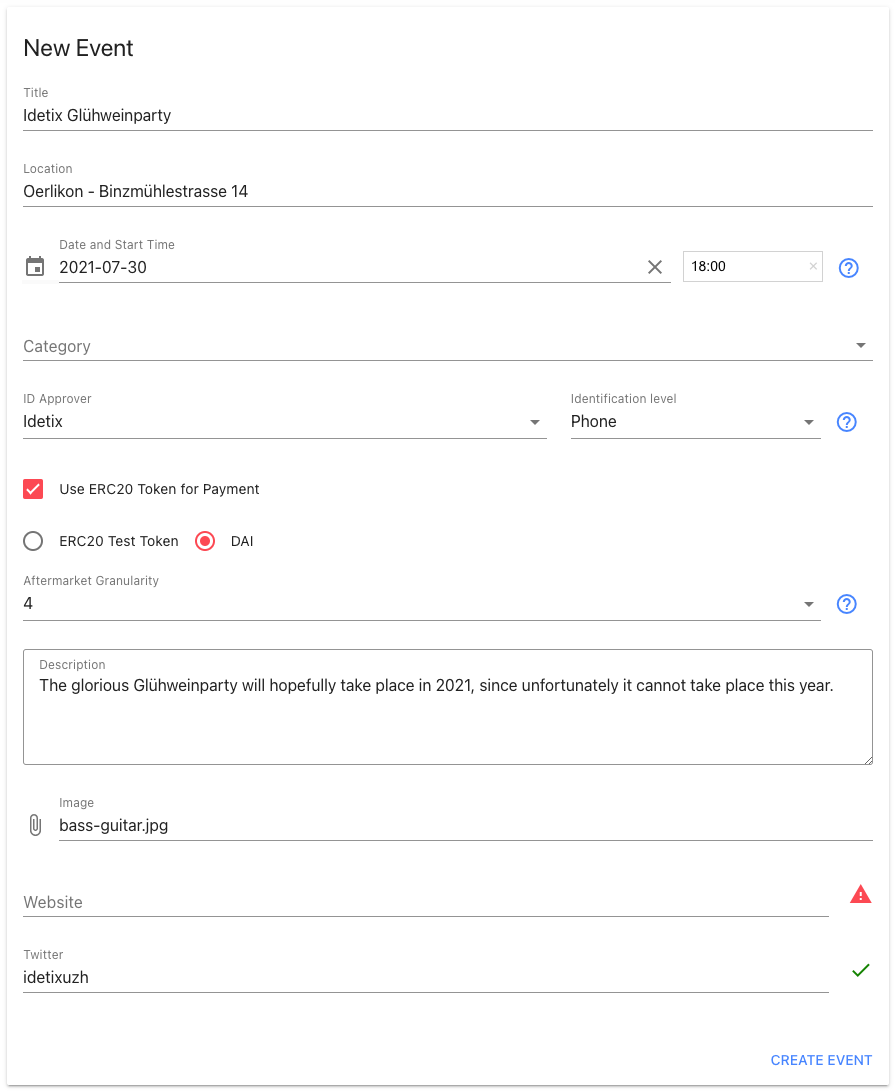
\includegraphics[width=15cm]{images/host-event-form.png}
    \caption{Event Creation Form \protect}
    \label{img:host-event-form}
\end{figure}

\subsection{Event List}
The event list is a simple view that contains a list of event cards. These event cards each contain the metadata for that event and some information directly from the blockchain, i.e. the maximal number of tickets per person, the currency or the identity approver that is required to buy a ticket. For more information about an event, a click on the card will route to the event summary view.

\subsection{Event Summary}
The event summary view contains multiple components that offer an overview of the event, its tickets and their states. On top a slightly reconfigured event card to the card in the event list is shown. Here it shows also the event contract address and an edit button. Either the metadata or the maximal number of ticket per person can be changed. Upon clicking the edit button, the host is prompted what to change and the according component is shown to make such a change. When changing the metadata, an event creation form is displayed, that is filled with the current metadata. This form can be edited and then submitted. In the form, only the image input is not filled out with the current data, since it is stored in a base64 representation. If no new image is uploaded in this input field, the current image is just used again.

After a change to the event or when canceling the attempted change, the event summary is shown again with the updated data, depending whether an actual change was applied. Below the event card, the tickets of the event are summarized. On the left is a list of ticket types that exist for that event and when selecting a ticket, the information about this ticket is shown on the right. This information contains data from the blockchain and metadata that is fetched from IPFS. It shows details such as whether the ticket is fungible or non-fungible, the price, the amount of tickets that have already been sold and the finalization time. This finalization time specifies the time, when tickets can no longer be bought or sold.
Tickets with a presale show further the status of this presale. Either, the presale has already passed, or otherwise, an estimated time is shown, when the presale presumably will end.

Additional to that the blockchain information of a ticket, the metadata as of Listing \ref{ticket-metadata-json-schema} are shown, i.e. title, description and the seating color. The latter may then directly be used to visualise what seats this type contains on the seating plan that is shown directly below.

To add a new ticket type to the event, this ticket summary component holds a button on the top right, which opens a ticket form. In this form, the host can set the metadata for a new ticket type as desired. There are just a few restrictions that arise from properties of the event or already existing ticket types, such as already used seats in the seating plan component, that may not be used for another ticket type. When saving a category, the selected seats of the seating plan component together with the filled out information in the ticket form are pre-saved and added to a list below as in Figure \ref{img:host-seating-plan}. A new submit button is now shown. With this button, the ticket types are created in one invocation on the event contract. By our design choice in the smart contracts, ticket types with a presale require a separate invocation. This means, that if the pre-saved tickets contain both tickets with a presale and tickets without a presale, two invocations are required.

\begin{figure}[H]
    \centering
    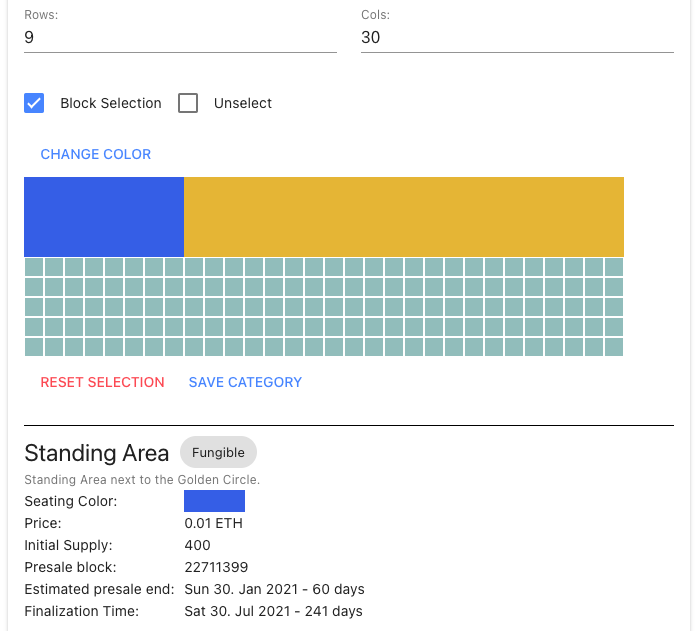
\includegraphics[width=14cm]{images/host-seating-plan.png}
    \caption{Seating Plan \protect}
    \label{img:host-seating-plan}
\end{figure}

Currently we allow changes to the ticket metadata in our smart contracts. However, since in our design the seat mapping of a ticket type is also stored in the metadata, we do not provide such functionality in the host-client to prevent duplicated seats in the seating plan. We address this further in the future work section \ref{future-work-ticket-metadata-change}.

\subsection{Identity Approver Registration}
As extension to the host client application, two views are included supporting basic interaction with the identity smart contract. The identity approver registration view contains a form to easily register as an approver with the supported methods, website and twitter. The website and twitter input fields also trigger a check for the trust certificates as in the event creation form.

\subsection{Identity Approval}
The identity approval form allows to easily store the verification level of an account on the identity smart contract.


%After connecting with an account, the first page stores the active account, its balance and a full \textit{web3} instance in the Vuex store. As soon, as the landing page receives that information,  --> to implementation part